\subsection{Pemartisian Basis Data}

Pemartisian (atau \textit{sharding}) merupakan sebuah cara untuk membagi basis data yang besar menjadi bagian-bagian yang lebih kecil \parencite{dataIntensiveApplications}. Beberapa partisi dapat disimpan pada \textit{node} yang berbeda, sehingga dataset yang besar dapat didistribusikan pada beberapa media penyimpanan. Selain itu, beban \textit{query} juga dapat didistribusikan pada beberapa mesin yang berbeda.

Pemartisian dapat dibagi menjadi dua, yaitu pemartisian horizontal yang membagi data berdasarkan baris dan pemartisian vertikal yang membagi data berdasarkan kolom.

Tujuan dari pemartisian data adalah untuk menyebarkan data dan beban secara adil kepada \textit{nodes} yang berbeda. Untuk itu, pendekatan untuk membagi data juga menjadi hal yang penting dalam partisi data. Berikut adalah beberapa pendekatan yang umum digunakan:

\begin{enumerate}
    \item Partisi berdasarkan kunci, seperti judul buku yang berawalan A-E, F-J, dan seterusnya. Meskipun begitu, perlu diiperhatikan apakah distribusi kunci tersebar secara merata.
          \begin{figure}[htbp]
              \centering
              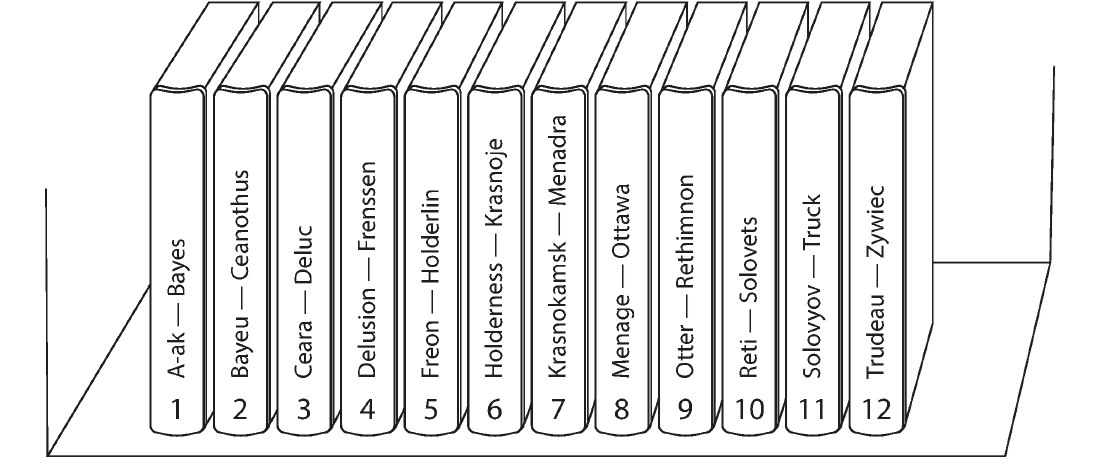
\includegraphics[width=0.8\textwidth]{resources/chapter-2/partition-by-key-range.png}
              \caption{Pemartisian berdasarkan rentang kunci \parencite{dataIntensiveApplications}}
              \label{fig: partition-by-key-range}
          \end{figure}

    \item Partisi berdasarkan hash kunci. Fungsi hash yang baik dapat mengubah distribusi kunci yang tidak simetris menjadi merata.
          \begin{figure}[htbp]
              \centering
              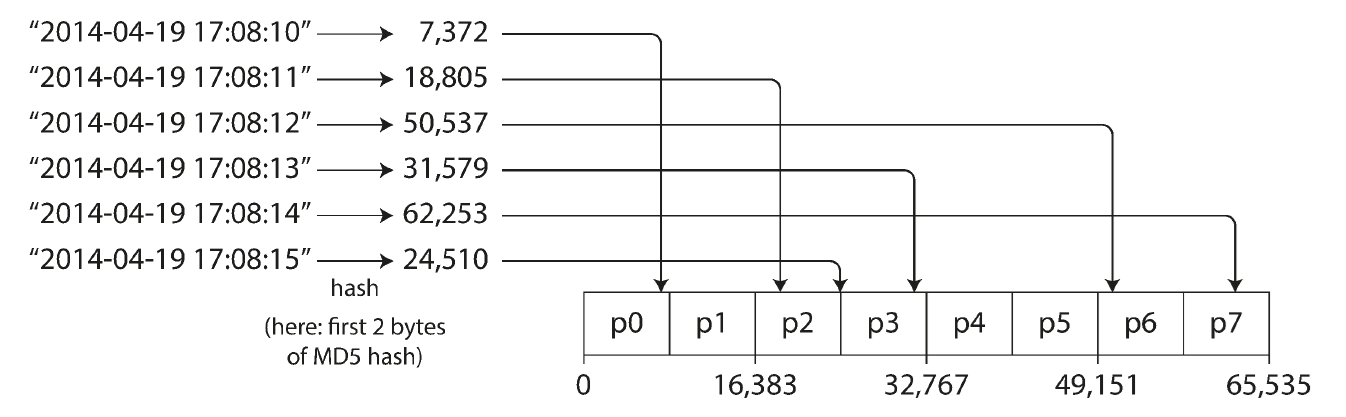
\includegraphics[width=0.8\textwidth]{resources/chapter-2/partition-by-hash.png}
              \caption{Pemartisian berdasarkan hash \parencite{dataIntensiveApplications}}
              \label{fig:partition-by-hash}
          \end{figure}

\end{enumerate}